\documentclass[letterpaper,twocolumn,10pt, anonymous]{article}
\usepackage{usenix2019_v3}

\usepackage{amsmath}
\usepackage{filecontents}
\usepackage{tikz}
\usepackage{xspace}
\usepackage{listings}
\usepackage{xcolor}
\usepackage{textcomp}
\usepackage{graphicx}
\usepackage{caption}
\usepackage{subcaption}
\usepackage{todonotes}
\usepackage{multirow}
\usepackage{booktabs}
\usepackage{paralist}
\usepackage{enumitem}
\usepackage{tabulary}
\usepackage{prettyref}
\usepackage{verbatim}
\usepackage{balance}

%-------------------------------------------------------------------------------
\begin{document}
%-------------------------------------------------------------------------------


\newcommand\tocttou[0]{ToCtToU\xspace}
\newcommand\tiktok[0]{TikTok\xspace}

\newrefformat{cha}{\hyperref[#1]{Chapter~\ref*{#1}}}
\newrefformat{sec}{\hyperref[#1]{Section~\ref*{#1}}}
\newrefformat{sub}{\hyperref[#1]{Section~\ref*{#1}}}
\newrefformat{tab}{\hyperref[#1]{Table~\ref*{#1}}}
\newrefformat{fig}{\hyperref[#1]{Figure~\ref*{#1}}}
\newrefformat{line}{\hyperref[#1]{line~\ref*{#1}}}
\newrefformat{lst}{\hyperref[#1]{Listing~\ref*{#1}}}
\newrefformat{pat}{\hyperref[#1]{Patch~\ref*{#1}}}
\newrefformat{alg}{\hyperref[#1]{Algorithm~\ref*{#1}}}

\newcommand\TODO[1]{\noindent{\color{green} {\bf \fbox{TODO}} {\it#1}}}

%don't want date printed
\date{}

% make title bold and 14 pt font (Latex default is non-bold, 16 pt)
\title{\Large \bf Kernel TOCTTOU Protection}

%for single author (just remove % characters)
\author{
{\rm Anonymous}\\
Your Institution
% copy the following lines to add more authors
% \and
% {\rm Name}\\
%Name Institution
} % end author

\maketitle

%-------------------------------------------------------------------------------
\begin{abstract}
%-------------------------------------------------------------------------------
Your abstract text goes here. Just a few facts. Whet our appetites.
Not more than 200 words, if possible, and preferably closer to 150.
\end{abstract}

\section{Design}

\tiktok is designed to maintain a single invariant: 
\emph{Every read to a userspace object by a syscall throughout its lifetime 
will read the same value}.
By construction, the invariant guarantees that double-fetches in syscall
code will read the same data, eliminating \tocttou bugs. 
\tiktok maintains the invariant by tracking \emph{snaphots} of the data
when first accessed, lazily making \emph{copies} when the data is concurrently 
written and accessing the correct copy on subsequent reads.
Copies are only maintained during the syscall's lifetime, and are released as 
soon as no syscall needs it.
Consequently, each page has a single copy while no syscalls are running.

\tiktok's implementation leverages the protection mechanisms provided by 
existing virtual memory implementations. 
On modern platforms, virtual memory protection is set up by the OS at
page-granularity by setting bits in page-table entries.
These permission bits are checked by the hardware on memory access, 
efficiently enforcing that the permissions are respected, or raising 
a fault when they are not.
Therefore, \tiktok implements its invariant at a page-granularity, not object 
granularity: when a syscall reads from userspace, every page touched by that 
read are covered by the invariant, not merely the bytes read.
As a side-effect of this implementation, \tiktok cannot differentiate between
accesses to different parts of a page, and incurs overhead on false sharing
within a page.

For an object spanning multiple pages, \tiktok's design sequentially 
protects each page before reading from it, and does not introduce 
new vulnerabilities. 
The leading pages containing the object are protected before the
later pages, allowing an attacker to potentially modify the later 
pages before the syscall first reads them.
However, the attacker is prevented from modifying any of these pages
after the syscall's first read, ensuring that double-fetches respect
the invariant.
If the syscall code contains a \tocttou bug, the modification will
be visible to the first fetch itself (which is used for checking for 
validity of the data) and will lead to the data being rejected 
straightaway.

A major design goal for \tiktok is to allow concurrently access to pages
by user/kernel code running concurrently to a syscall which reads from 
the same pages.
To ensure that writes to pages do violate the invariant, \tiktok
must maintain multiple copies of a page.
Particularly, for each syscall which has accessed a page, \tiktok
must maintain a snapshot of its contents from when the page was first 
read by the syscall.
A separate copy of the page will be used for concurrent reads and writes,
updating the page as seen from userspace.
When multiple syscalls read from the same page, and there are no writes
to the page between the times when each first accessed the page, 
the snapshots of the page for these syscalls may correspond to a 
single copy.

\subsection{Page state machine}

\begin{figure*}[]
  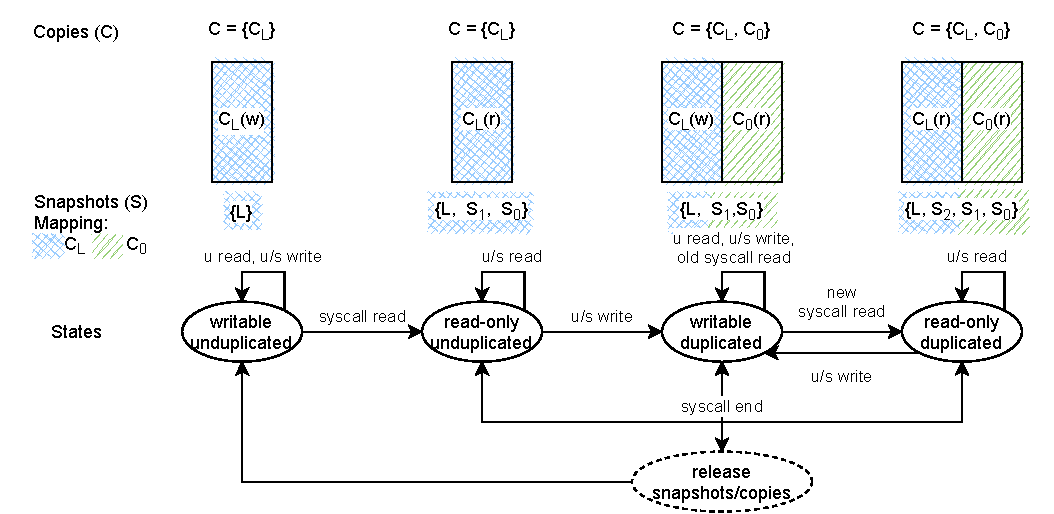
\includegraphics[width=\linewidth]{img/tiktok_states.pdf}
  \caption{State diagram for a page in \tiktok}
  \label{fig:tiktok_states}
\end{figure*}

To track multiple versions of the contents of a page when being concurrently 
accessed by numerous threads, from userspace or during a syscall,
\tiktok implicitly maintains a per-page state machine for every single 
user page.
For each page, its corresponding state machine tracks snapshots for currently 
executing syscalls which have read it, copies of the page, and the mapping 
between the two necessary for providing the correct contents to subsequent reads 
by these syscalls.

\autoref{fig:tiktok_states} shows the state machine for a single page.
At every state, the page has two associated sets:
\begin{inparaenum}[\itshape i\upshape)]
  \item the copies set $C = \{C_L, C_0, \dots\}$ holds multiple copies of the page over time, and
  \item the snapshots set $S = \{L, S_0, S_1, \dots\}$ tracks logical versions of the page, each corresponding to one executing syscall and mapping to a copy. 
\end{inparaenum}
Reads from kernel code in a syscall use the copy corresponding to its snapshot.
Writes from user/kernel code and reads from userspace access the latest 
copy, which is mapped in process' address spaces.
\TODO{Should I formally define this mapping?}
All other copies are read-only, and are used for providing snapshots to syscalls.
In the following paragraphs, we describe how the state machine for a single page 
transistions between its states, what triggers each transistion, and what 
changes are made to the copies and snapshot sets on a transistion.

\paragraph{State 0}
A page starts as (writable, unduplicated). 
At this stage, there is a single writable copy $C_L$ and a single snapshot $L$. 
All processes where this page is mapped have unrestricted userspace read and write 
access, and unrestricted kernel write access.
The remaining operation, a read from kernel code, triggers a transistion to 
the next state.

\paragraph{State 1}
The page transistions to (read-only, unduplicated) state as soon as a syscall 
reads from it. 
\tiktok first marks the page's latest copy $C_L$ read-only in all processes, 
restricting writes to it but allowing concurrent reads to continue.
A new snapshot, $S_0$ linked to this syscall is allocated for this page.
For the rest of its lifetime, this syscall will only read from this snapshot.
Both snaphots $S_0$ and $L$ refer to the same copy $C_L$ (shown by the 
blue cross-thatch in \autoref{fig:tiktok_states}).
Prior to any writes to this page, any other syscalls which also read the page  
get their own snapshots (e.g. $S_1$) all pointing to the single copy $C_L$.
The page's read-only status causes the hardware to fault on any write,
notifying \tiktok to transistion the page to the next state.

\paragraph{State 2}
A page in State 1 transistions to (unmarked, duplicated) on any write.
\tiktok duplicates the latest copy $C_L$, creating a new copy $C_0$ holding
the pre-write contents of the page.
\tiktok moves all snapshots ($S_0$ and $S_1$) previously pointing to 
$C_L$ to now point to the new copy $C_0$ (shown by green hachure in 
\autoref{fig:tiktok_states}). 
Thereafter, the latest copy $C_L$ is made writable, and the triggering write 
is retried. 
Note how, at this state, any reads using the snapshots $S_0$ or $S_1$ reads 
from the unmodified copy $C_0$ while writes directly affect $C_L$.

\paragraph{State 3}
A separate syscall subsequently reading the page in State 2 transistions 
it to (read-only, duplicated) state. 
The new snapshot, $S_2$, points to the latest copy $C_L$.
On a write, the page will be duplicated and this snapshot 
will point to the new copy (similar to that in state 2).

\paragraph{Releasing snapshots}
\tiktok uses snaphots to enable a syscall to read the same data from a page 
during its lifetime and releases snapshots when syscalls complete. 
When a snapshot is released, \tiktok may also release its mapped copy.
For a snapshot mapped to the latest copy $C_L$, \tiktok cannot free the copy
since userspace is using it.
In this case, the page is in states 1 or 3, and $C_L$ is read-only.
If no remaining snapshot is mapped to $C_L$, \tiktok makes the 
page writable, moving to states 0 or 2 from states 1 or 3 respectively. 
Any other duplicate $C_i$, \tiktok frees the copy along with the 
last snapshot which mapped to $C_i$.
If the page was in state 2, $C_L$ was writable and unmapped by any snapshot,
so \tiktok changes the page to state 0.
If the page was in state 3, $C_L$ was read-only and mapped by some other
snapshot, so \tiktok moves the page to state 1.

\TODO{Discuss how Midgard would help}
\tiktok assumes that syscalls do not both read and write to the same user data. 
There are particular syscalls, however, which rely on such behaviour, and 
are not instrumented.

Fake citation for compilation~\cite{silberschatz2018operating}.

\bibliographystyle{plain}
\bibliography{TikTok}

%%%%%%%%%%%%%%%%%%%%%%%%%%%%%%%%%%%%%%%%%%%%%%%%%%%%%%%%%%%%%%%%%%%%%%%%%%%%%%%%
\end{document}
%%%%%%%%%%%%%%%%%%%%%%%%%%%%%%%%%%%%%%%%%%%%%%%%%%%%%%%%%%%%%%%%%%%%%%%%%%%%%%%%

%%  LocalWords:  endnotes includegraphics fread ptr nobj noindent
%%  LocalWords:  pdflatex acks
